\subsection{The Maximum Pick-Up-Sticks (MPUS) Algorithm}

As proposed by "Applegate et al."'s paper, we can build an algorithm for finding whether a pattern is a strip-rule pattern and if so, finding an SRRL that generates it.

\subsubsection{The Pick-Up-Sticks (PUS) Algorithm.}

The Pick-Up-Sticks algorithm of \cite{ACJKLW07}
 is an algorithm for generating a SRRL of a pattern P if such a list exists. The idea is to pick up monochromatic rows and columns in order to build the SRRL backwards. Every time we pick a row or column, we color it gray.

Let $P$ be a black and white pattern. We define a column or row in P as being pseudo-monochromatic if it is composed of only gray and white cells or black and gray cells. Note that monochromatic columns and rows are also pseudo-monochromatic.

The Pick-Up-Sticks algorithm builds an SRRL as follows:

While there are still
black cells, choose a pseudo-monochromatic column or row and color all its cells gray. After a row or column is colored gray, add a rectangle that corresponds to covering that row or column with whatever non-gray color was left in that row or column to the beginning of our SRRL.
Note that, in our problem definition,
 we begin applying SRRLs with a white grid, so we can stop
picking up sticks when no black cells exist.
If, on the other hand, we modify the problem to begin with a grid of some
third color, we would only stop picking up sticks when all cells are gray.
There may be a difference of one rule between the optimum solutions to these two
problems (white grid or some third color grid) with the same target pattern.
For the sake of symmetry, from now on we use this {\em modified version}
of the problem. The method works with minor modifications for
the original version.

The algorithm may not succeed,
as it may not find a pseudo-monochromatic column or row.
If the algorithm does end in a all-gray grid,
%the algorithm has found a SRRL for the pattern $P$. If not, $P$ is not a strip-rule pattern. For the successful case,
the algorithm has "picked up" the rectangles of the SRRL in reverse order. Figure~\ref{fig:pick_up_sticks_example} gives a representation of one possible execution of the Pick-Up-Sticks algorithm and Fig.~\ref{fig:pick_up_sticks_srrl} shows the generation of the original pattern from the resultant SRRL.

\begin{figure}[h]
\centering
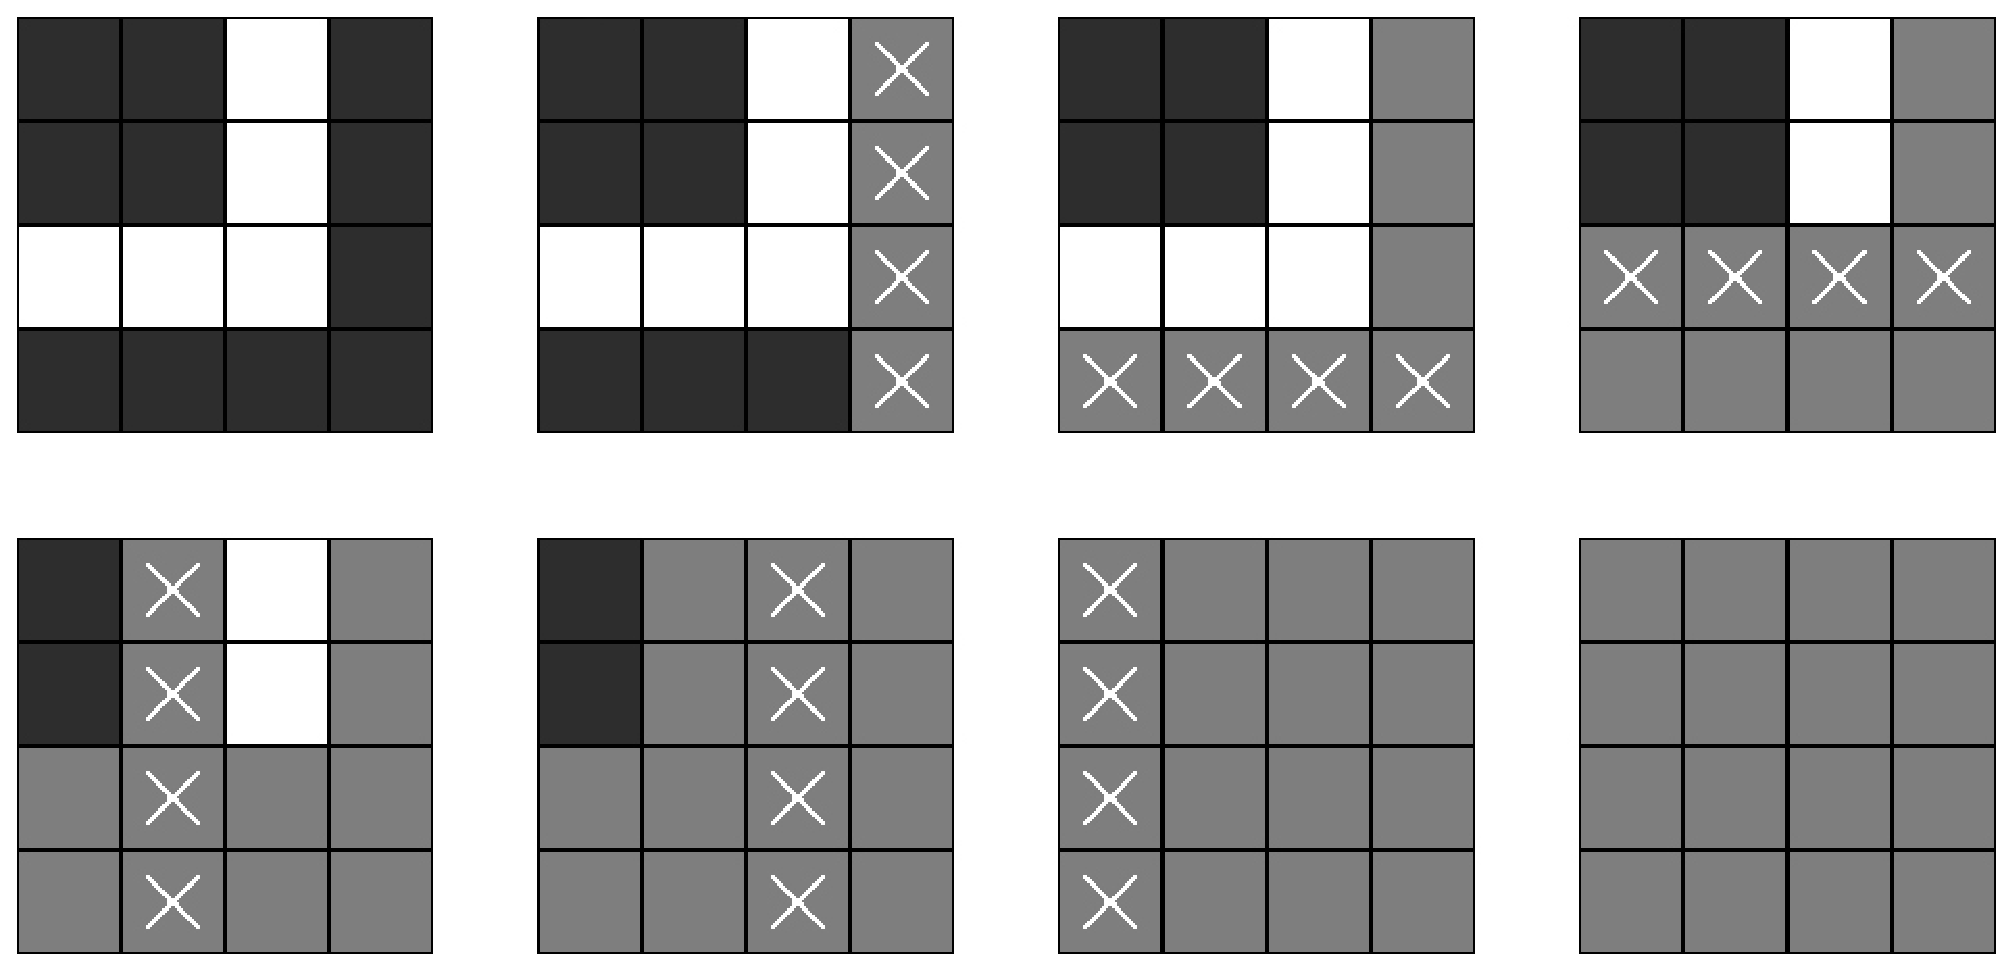
\includegraphics[width=10cm]{pick_up_sticks_example}
\caption{The execution of the Pick-Up-Sticks algorithm on a strip-rule pattern.}
\label{fig:pick_up_sticks_example}
\end{figure}

\begin{figure}[h]
\centering
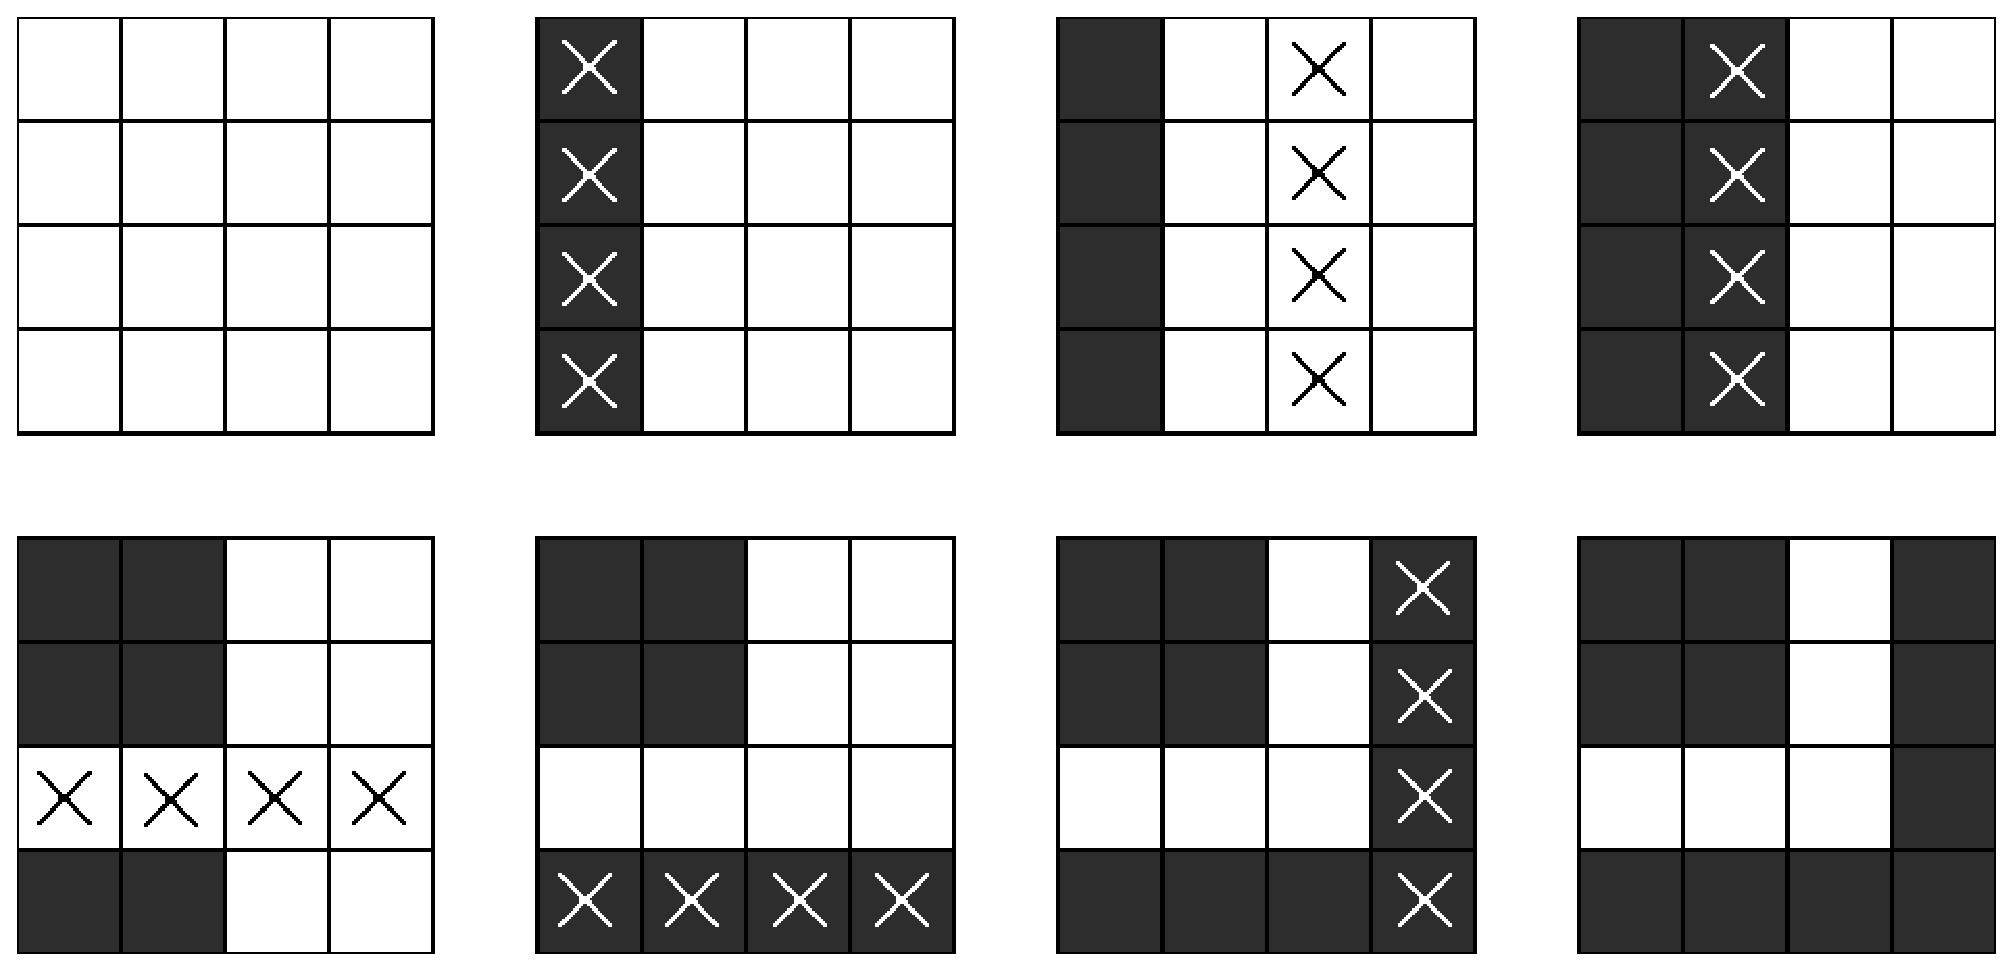
\includegraphics[width=10cm]{pick_up_sticks_srrl}
\caption{The SRRL generated by the execution of the MPUS algorithm on the pattern of the Figure~\ref{fig:pick_up_sticks_example}}
\label{fig:pick_up_sticks_srrl}
\end{figure}

The Pick-Up-Sticks algorithm is guaranteed to generate an SRRL if one exists
\cite{ACJKLW07} (included in Appendix, Subsection \ref{corr_pus}), but it is not necessarily the optimal SRRL of minimum length. At any stage of the algorithm there will be more than one option on which row or column to pick up. Different choices can lead to different sizes of SRRLs. In the next sections we will discuss on how "Applegate et al."'s paper narrows down the number of choices for each stage in order to find the minimal SRRL.

\subsubsection{Improving by Picking Maximal Sticks.}

One important observation by "Applegate et al."'s paper on the Pick-Up-Sticks (PUS) algorithm is that there can be no harm in always using maximal strip-rules. A maximal strip-rule is a strip-rule that picks up a maximal contiguous sequences of pseudo-monochromatic rows or columns. Following \cite{ACJKLW07},
we call such a contiguous sequence a {\em block}.

This is possible because replacing a non-maximal strip-rule by the maximal one that contains it does not affect the pseudo-monochromaticity of any later rule.

Hence, we may always use the Maximal Pick-Up-Sticks (MPUS) algorithm instead of the Pick-Up-Sticks (PUS) algorithm. In this new algorithm, once we choose the pseudo-monochromatic column to pick, we pick the maximal contiguous set of pseudo-monochromatic columns that contains it.
